
\chapter{Introduction}

\section{Introduction}
\subsection{Motivation}
\label{sec:motivation}
Mesenchymal stem cells might hold the promise for a great leap forward in future regenerative medicine therapies. \\
MSC can give rise to various cells found in fat- (adipocytes), cartilage- (chondrocytes), bone- (osteoblasts) and tendon-tissue (tenocytes) \cite{Barlow2008, Hass2011} and as such are important for development.
Furthermore, they are also critical to life-long regeneration of tissue, as they persist during adult life in different "niches", like the bone-marrow or in adipose tissue. Additionally, they can be isolated and cultured, albeit rare in frequency. Because of this versatility, their capacity for self-renewal and their robustness, research is being done to exploit this potential for medical applications. Baek and colleagues recently described a way of \textit{ex vivo} manipulating the MSCs' homing behaviour before injecting them back in the donor, which stimulates migration towards injured tissue and could in the future improve recovery from myocardial infarction \cite{Baek2011}.  Additional proposals for novel applications span the fields of spinal injuries\cite{Goldschlager2010}, Multiple Sclerosis \cite{Planchon2018}, Alzheimer's Disease \cite{Han2018, Hao2012} and Diabetes \cite{Evangelista2018}.  While the promises that MSCs hold might be worthwhile, translation has been challenging. Despite the prospect of a medical revolution, currently there is no FDA approved MSC therapy available, as past proposals have been shown to either ineffective or dangerous. For example, Amariglio et al. report of a dramatic account of a boy developing multiple ectopic brain tumours as a result of a faulty stem cell therapy \cite{Amariglio2009}. Such downsides show that we need to increase our basic understanding of MSCs so that we can avoid the hazards and harness the benefits in the future.\par

The historic paradigm in cell biology that a system is described only through its biochemical status has come into question during the last years. We now know that mechanical forces, which cells experience \textit{in vivo}, influence their behaviour \cite{Hao2015}. Mechanosensing, the ability to sense forces, is a contributing factor in many cellular contexts from migration to differentiation and self-renewal. In a landmark study, Engler and colleagues\cite{Engler2006} showed that MSCs can decide on their cell fate only due to physical substrate stiffness. This study is one of many more following accounts showing that there is new, decisive knowledge in studying biophysical interaction between cells and their physical surroundings.\par

However, it is not fully understood what pathways are involved in mechanosensation of MSCs and how they regulate stem cell behaviour. More recently, the membrane-bound mechanosensitive ion-channel \Piezo{} has been described \cite{Coste2010}. The discovery marked a turning point in mechanobiology as it described the first and long sought-after eukaryotic mechanosensitive ion channel \cite{Sharif-Naeini2015}. Since then, many studies have corroborated the idea of \Piezo{} belonging to a family of receptors who have already been predicted to exist since 1950 \cite{Katz1949}. While we now know that \Piezo{} is involved in neural stem cell differentiation \cite{Pathak2014} and vascular development \cite{Ranade2014}, it is not fully understood how \Piezo{} influences MSC behaviour. \par
In this work, we investigate the importance of \Piezo{} in MSC mechanosensing and shed light on its influence regarding ECM turnover and differentiation.

\section{Theory}

\subsection{Bone Marrow-derived Mesenchymal Stem Cells}

Mesenchymal stem cells (MSCs) are characterized by three different properties: First, they hold the potential to differentiate into any tissue that originates from the mesenchymal germ layer. This set of cell types includes osteocytes (bone), chondrocytes (cartilage), adipocytes (fat-tissue) and tenocytes (tendon) \cite{Ng2008}. Second, they hold the potential to self-renew, meaning they can give rise to identical cells. And third, they expose a non-specific set of markers like CD49a, CD105 and CD146 amongst others \cite{Bianco2013}. Furthermore, there is a growing body of evidence that attributes an immunomodulatory effect of MSCs on injured or inflamed sites, which, when harnessed in clinical application, could relate to better outcome in medical therapies \cite{Caplan2011, Hass2011}.
While there are differing anatomical sources where mesenchymal stem cells can be isolated from, including the umbilical cord and adipose tissue \cite{Barlow2008, Hass2011} in this work we focus on human bone-marrow derived mesenchymal stem cells and from now on will refer to them as mesenchymal stem cells (MSCs). 

It is important to note, that in this project, the used cells are \textit{bona fide} mesenchymal stem cells. A more inclusive description of the cells at hand would be bone-marrow derived stem/stromal cells. For simplicity, however, we will call our cells MSCs for the rest of this work. For further reading on the relation between bone-marrow derived mesenchymal stem cells and bone-marrow stromal cells consult \cite{Bianco2013}.

\subsection{Mechanobiology of MSCs}

\begin{figure}
	\centering
	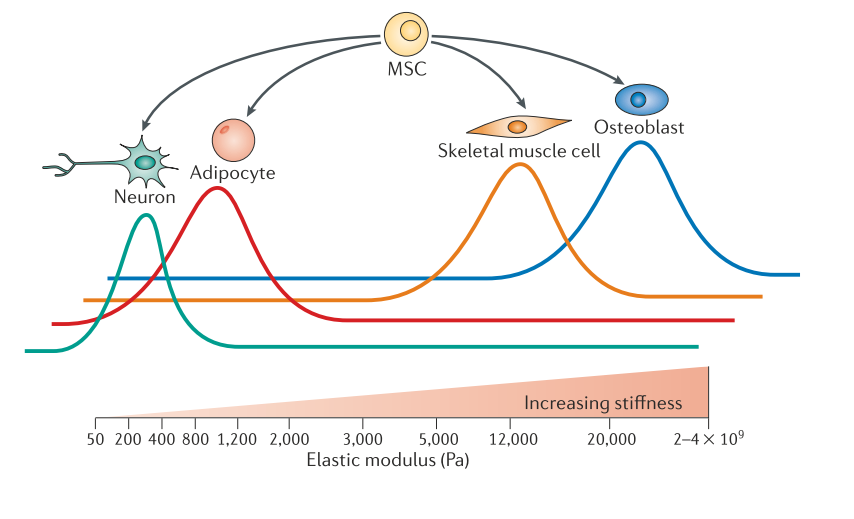
\includegraphics[width = 0.8\textwidth]{STIFFNESS_DIFFERENTIATION.PNG}
	\caption{MSCs show different cell lineages emerging along a continuous substrate stiffness spectrum. Adapted from \cite{Halder2012}.}
	\label{fig:StiffDiff}
\end{figure}

MSCs have great potential for medical therapies. As such there is an interest in finding out the underpinning mechanisms governing MSC behaviour. During the last two decades, there was a lot of work done, bringing to light how the mechanobiology of MSC regulates differentiation and development (see Fig. \ref{fig:StiffDiff}). For example, there is evidence that MSCs are able to distinguish between various types of forces. MSCs differentiate into different lineages, depending whether they are exposed to compressive forces, which lead to chondrogenic differentiation, or tensile forces, where there are more osteogenic differentiation markers observed.\cite{Kearney2010, Saitoh2000} There is also an emerging role of chemical signals expressing their role in a complex interplay with biophysical signals to regulate development. Ruiz and colleagues suggest this in their work, where they exposed multicellular MSC aggregates to media, that favours both adipogenic and osteogenic lineage choice. They showed differing differentiation of MSCs inside the aggregates depending on their relative location and the corresponding stress level. Cells that were in the outer layer, experienced more stress and showed more osteogenic differentiation, compared to cells in the middle, lower stress region, which showed signs of adipogenic differentiation \cite{Ruiz2008}. The distribution of differentiation over the aggregate resembled the primitive structure of a bone, with a middle spongy, fatty marrow surrounded by a calcified outer shell. Another example are avian embryos that when completely immobilized show largely deficient development in bones and muscles \cite{Castillo2010}. This indicates how mechanical forces might contribute to complex developmental processes.\\ 

With more insight generated, it becomes increasingly important to understand the pathways mediating mechanosensation. YAP\textbackslash{}TAZ for example is shown to be a potent mechanotransducer in MSCs \cite{Halder2012}. YAP\textbackslash{}TAZ is part of the Hippo Pathway and has been shown to mediate mechanotransduction through changing intracellular localization (nuclear or cytosolic). Coste and colleagues showed that YAP\textbackslash{}TAZ mediates mechanosensation of physical cues, like ECM stiffness, as they observed that, when the cell is seeded on stiff substrate and is showing signs of osteogenic differentiation, YAP\textbackslash{}TAZ is localized preferably inside the nucleus. They were also able to show that altered YAP\textbackslash{}TAZ localization was able to override those physical cues suggesting a causal relationship between mechanosensation and YAP\textbackslash{}TAZ \cite{Coste2010}.



\subsection{\Piezo{}}

\begin{figure}
	\centering
	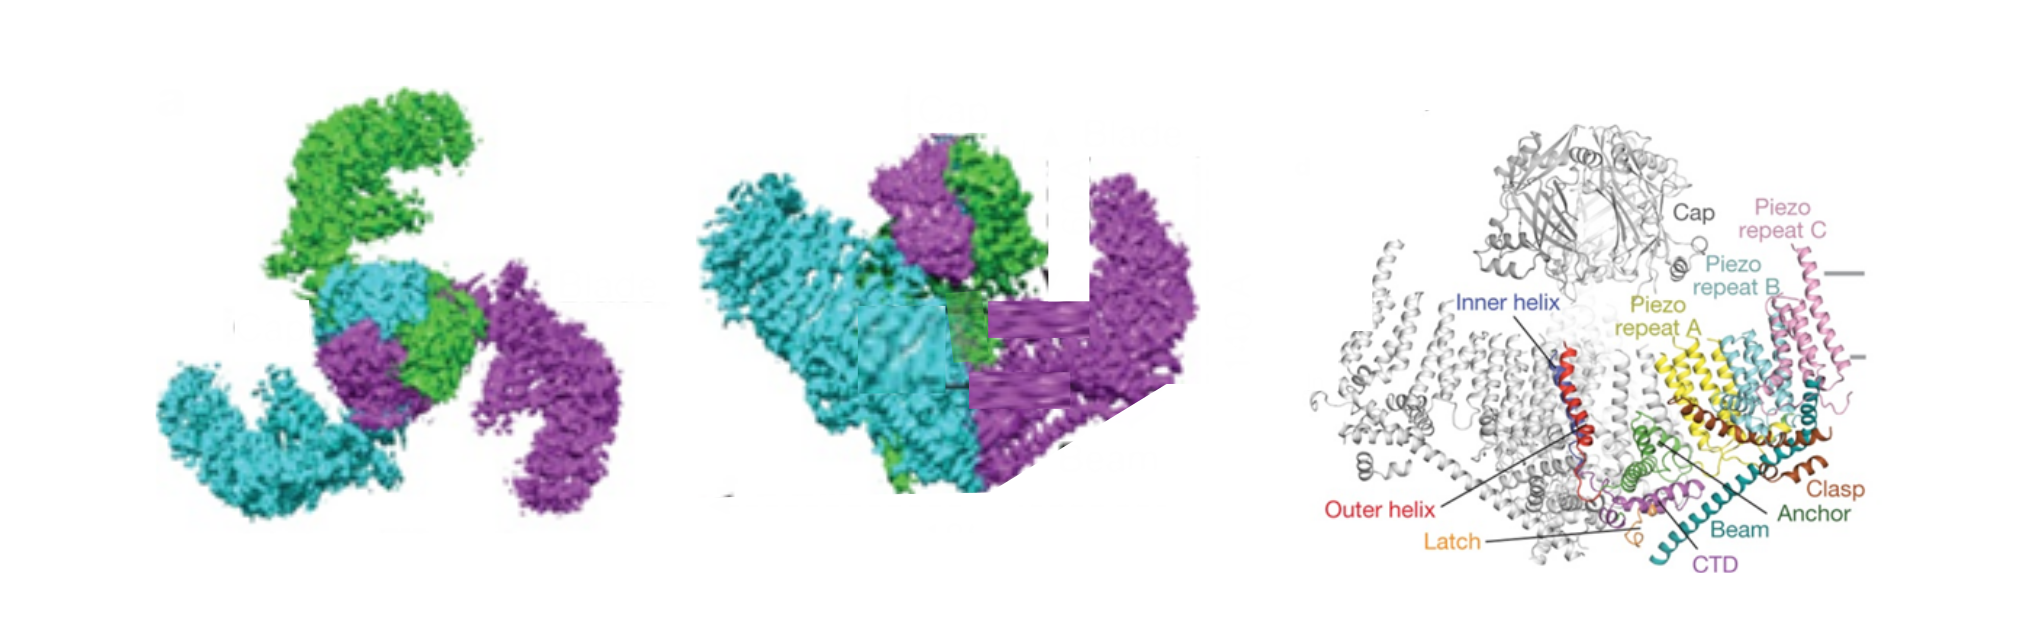
\includegraphics[width=0.9\linewidth]{PiezoMolecule.png}
	\caption{Molecular structure of \Piezo{} as assessed by cryo-EM analysis. Top (left) and side (middle) view of \Piezo{} and cartoon representation of \Piezo{} with important domains highlighted (right). Adapted from \cite{Saotome2018, Zhao2018}.}
	\label{pic:Piezo}
\end{figure}

\Piezo{} and \textsc{Piezo2} are the only known members of the \textsc{Piezo}-family. The protein family is genetically and structurally unique, as the similarity to other proteins are minimal \cite{Coste2010}. \Piezo{} can be found in various tissues and cell types throughout the body and constitutes the mechanosensitive homo-trimeric cation channel \Piezo{} \cite{Zhao2018}. \Piezo{} is evolutionary conserved as homologues span the whole division of multicellular animals. Intriguingly, the uniqueness also translates to the architecture of the channel as shown in work done by Saotome and colleagues giving great insight into \Piezo{}-structure using cryo-EM analysis \cite{Saotome2018}. The large channel comprises a central pore in the middle with a three-bladed propeller like structure facing the extracellular space (see Fig.~\ref{pic:Piezo}).\\
The exact trigger of activation is still matter of an on-going debate. However, when activated \Piezo{} switches into an open state where it allows \calcium{} and other cations to enter the intracellular space, before reverting into an inactive state, where the channel is non-responsive to stimuli. After a relaxation period, the channel switches back to a responsive, closed state. While the exact activation mechanism remains elusive, there is evidence for the mechanotransductory chain starting with force-mediated bending of blades which then transmits the tension over anchor/beam region, leading to the opening of a previously allosterically closed inner portion of the cation channel \cite{Zhao2018}. This hypothesis is corroborated by findings that blades exhibit flexibility over many different bending modes, which supports the notion of the blades being the mechanosensory unit of the channel \cite{Ge2015}.  Research on mechanosensitive ion channels and \Piezo{} relied until recently on physical activation techniques, like application of physical forces or the patch clamp technique. Alternatively, \Piezo{} can be activated by a small pharmacological \Piezo{}-agonist, called \Yoda{} (a nod towards movie director George Lucas’ use of “the Force”). \Yoda{} has been shown to chemically activate \Piezo{} by acting as a molecular wedge, without eliciting a similar response in other channels \cite{Lacroix2018, Syeda2015}. Therefore, \Yoda{} can be used to study the influence of \Piezo{} in an isolated design \cite{Botello-Smith2019}.


